\documentclass{article}
\raggedright
\usepackage{graphicx}
\usepackage[a4paper,hmargin=25mm,bmargin=30mm,top=20mm]{geometry}
\begin{document}
\begin{center}
	\textbf{\LARGE Dinesh J}
	\rule{\textwidth}{0.5pt}
\end{center}	
S$/$O Jayanna J, \hspace{6.7cm} Contact No.-$8431619464$\\
Sri Veerabhadreshwara Oil Mill,\hspace{4.3cm}  Email Id - dineshj.dini@gmail.com\\
\#427, Barandur(P), \\Bhadravathi(T),Shimoga(D), \\  Karnataka.\\
PIN- $577301$\\
\begin{figure}[h]
	\begin{flushright}
			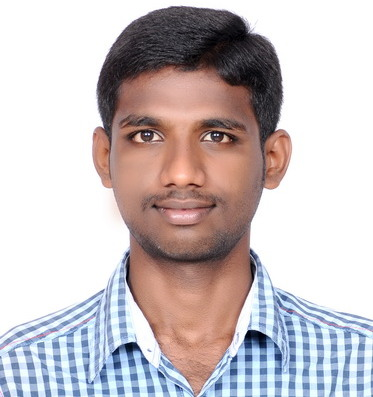
\includegraphics[scale=0.3]{Dinesh.jpg}
	\end{flushright}
\end{figure}
\textbf{OBJECTIVE:} \newline
To work in an organization where culture of freedom and working for initiatives is ensured, facilitating my contribution through thoughts and action to the company’s vision and thus achieve self development by playing a significant role in building the organization.
\newline

\textbf{EDUCATION:} \\ 

	\begin{tabular}{|p{2cm}|p{5cm}|p{5cm}|p{1cm}|p{2cm}|}
		\hline 
		\textbf{  Degree } & \textbf{ Institute} & \textbf{   Board University} & \textbf{Year} & \textbf{Result}\\ [0.5ex] 
		\hline 
		B.E.(ECE) & J.N.N College of Engineering,\hspace{1cm}Shimoga. & Vishveshwaraya Technological\hspace{.5cm} University, Belgaum. & 2015 & 71.33 \% \\
		\hline 
		Pre-university / XII(PCMB) &S.A.V Composite PU College, Bhadravathi. & Department of PU Education,	\hspace{.5cm} Karnataka. & 2011 & 80.16\% \hspace{1cm} (PCM 86 \%)	\\
		\hline 
		SSLC/ X & S.A.V High School, Bhadravathi. &Karnataka Secondary Education Examination Board. & 2009 & 	88.16 \%  \\				 
		\hline
	\end{tabular}
\newline \newline
\newline
\textbf{PROJECTS:}
\begin{enumerate}
	\item  \textbf{RAITA MITRA $–$ REMOTE AUTOMATION AND DATA MONITORING OF IRRIGATION
		SYSTEM}\\
			 This project aims to prevent burning out of the 3 Phase Motor Pump in farm land from different causes.\\
			 Presented this project and secured \textbf{1st Place} in \textbf{ IETE National Level} Project
			 Contest at Amrita University, Coimbatore.
			
			 \item \textbf{SMS BASED MOBILE VOTING SYSTEM}\\
			 The Voting system was made easily accessible by making it Mobile
			 Controlled.
			 
			 \item \textbf{HOME AUTOMATION}\\
			 This Project is designed and developed for controlling different home appliances through Android Mobile.
			 
\end{enumerate}
\textbf{TRAINING \& INTERNSHIP}
\begin{enumerate}
		\item \textbf{Vocational Training on Telecom Technologies}, BSNL, Shimoga, Karnataka.\\
		I attended the BSNL Advanced Telecom Training for one week where I not only got an overview to the range of telecommunication technologies, but also exposure to
		working/live telecommunication equipment deployed in BSNL.
		\item No internships\\	
\end{enumerate}

\textbf{RESEARCH PUBLICATIONS:}\\
  No research work done. \newline \newline
\textbf{TECHNICAL SKILLS:}
\begin{itemize}
	\item \textbf{Programming Languages} : C, ALP, Wiring, Embedded C
	\item \textbf{Software}			 \hspace{2.7cm}	: MATLAB, Energia, Multisim 
	\item \textbf{Hardware}			 \hspace{2.5cm}	: 8051,MSP430
\newline
\end{itemize}

\textbf{SOFT SKILLS:}
\begin{enumerate}
	\item Ability to work in a team. 
	\item Community group Involvement.
	\item Problem solving.
	\item Independent \newline
\end{enumerate}

\textbf{EXTRA CURRICULAR AND GROUP ACTIVITIES:}
\begin{itemize}
\item Conducted Hands-on Workshop on \textbf{MSP430 Microcontroller and Robotics} for Prefinal year students of Department of Electronics and Communication Engineering and
Telecommunication Engineering at JNNCE, Shimoga in which I trained 120 students
about Microcontroller and Robotics.\newline
\end{itemize}

\textbf{CO-CURRICULAR ACTIVITIES:}
\begin{enumerate}
	\item \textbf{1st  place} in \textbf{e-Yantra National Level Robotics Competition-2014} conducted by \textbf{IIT Bombay} under the sponsorship of MHRD, Government of India.
	\item \textbf{1st Place} in \textbf{‘National Project Contest Event’} held as a part of \textbf{2nd IETE Student Forum National Congress (ISFNC) 2015} at Amrita University organized by IETE Coimbatore Centre. 
	\item 	\textbf{2nd Place} in \textbf{National Level Circuit Debugging Competition} ‘CIRCUIT-O-FRENZY’ in DELTA 13.0 held at G M Institute of Technology, Davanagere, Karnataka.\newline
	
\end{enumerate}

\textbf{PERSONAL DETAILS:}
\begin{itemize}
	\item Father's Name: Mr Jayanna J
	\item Mother's Name: Mrs Kalpana
	\item Sex: Male
	\item Date of Birth: $25^{th}$ February $1993$
	\item Nationality: Indian
	\item Martial Status: Single \newline
\end{itemize}


\textbf{DECLARARION:}
I hereby certify that all the information provided above is true to the best of my knowledge.
\newline \newline \newline 
	\textbf{ Date:}		
	\today	\newline \\

\end{document}